\chapter{Paraphrase Evaluation}
\label{chap:paraphrase_evaluation}

 Paraphrase evaluation
    - automatic
        - syntactic 
        - semantic
    - human evaluation

% \subsection{Traditional Quantitative Paraphrase Evaluation}
% \label{subsec:traditional_quantitative_evaluation_measures}

% Evaluating paraphrases can be reduced to summarization or translation evaluation.
% The evaluation of paraphrases can be divided into syntactic and semantic approaches. 
% \citet{gohsen_captions_2023} normalized all metrics and averaged the semantic and syntactic scores separately.

\subsubsection{Syntactic Measures}
Syntactic evaluation metrics mainly focus on the n-gram overlaps~\citep{zhou_paraphrase_2021}. 
Common syntactic evaluation metrics include \acs{bleu}, \acs{rouge}-1, and \acs{rouge}-L.

\paragraph{\ac{bleu}}
\ac{bleu}~\citep{papineni_bleu_2001} was originally developed for machine translation~\citep{zhou_paraphrase_2021,anantha_pearson_metrics_2021}. 
\ac{bleu}'s basic unit of evaluation is a sentence. 
\ac{bleu} is based on precision, i.e.\ computing the fraction of generated n-grams $n\text{-}gram \in \mathcal{C}$ that appear in any reference text~\citep{kurt_pehlivanoglu_comparative_2024,palivela_optimization_2021,papineni_bleu_2001,anantha_pearson_metrics_2021}. 
To prevent inflated precision scores $p_n$ due to repetition of frequent tokens (e.g.\ "the"), \ac{bleu} introduces a clipping mechanism $Count_{match}(.)$ that caps the count of n-grams at their maximum reference frequency~\citep{papineni_bleu_2001}. 
Precision $p_n$ for $n \in \mathbb{N}_{>0}$ is given by \autoref{eq:bleu}.

\begin{equation}
    p_n = \sum_{\mathcal{C} \in \left\{ Candidates \right\}}\sum_{n\text{-}gram \in\mathcal{C}} \frac{Count_{match}(n\text{-}gram)}{Count(n\text{-}gram)}
\label{eq:bleu}
\end{equation}

The choice of $n$ determines what syntactic characteristic is evaluated.
Uni-grams are used to test adequacy, while longer n-grams are used to test fluency~\citep{papineni_bleu_2001}. 
The brevity penalty $BP$ from \autoref{eq:bleu_brevity_penalty} is applied to discourage excessively short candidates $c$~\citep{papineni_bleu_2001}.

\begin{equation}
    BP = \begin{cases}
        1 & \text{if } len(c) > len(r) \\
        e^{1 - \frac{r}{c}} & \text{else}
    \end{cases}
\label{eq:bleu_brevity_penalty}
\end{equation}

In order to compute the \ac{bleu} score from \autoref{eq:bleu} for more than one sentence, 
one (1) computes the clipped n-gram matches sentence by sentence, 
then (2) adds them across all sentences, 
and finally (3) divides the total clipped n-gram matches by 
the total number of unclipped n-grams in all candidate sentences~\citep{papineni_bleu_2001,cordeiro_bleu_2007}.

Combined scores across different n-gram orders are computed via the geometric mean, weighted uniformly (i.e.\ $w_n$) across different $n$~\citep{papineni_bleu_2001,banerjee_METEOR_2005}.
Combining precision $p_n$ (\autoref{eq:bleu}) and brevity penalty $BP$ (\autoref{eq:bleu_brevity_penalty}) leads to the final score in \autoref{eq:bleu_final}.

\begin{equation}
    \text{BLEU} = BP \cdot \exp\left(\sum_{n=1}^{N} w_n \cdot \log p_n\right)
\label{eq:bleu_final}
\end{equation}

\ac{bleu} disregards semantic similarity completely and therefore judges paraphrases only based on n-gram overlap. 
As such, it is generally recommended being supplemented with human evaluation~\citep{zhou_paraphrase_2021}.



% Its values range from 0 to 1 \citep{papineni_bleu_2001}.

% \ac{bleu} automatically penalizes n-grams appearing in the candidate text but not in the reference text, 
% as well as n-grams appearing more often in the candidate than in the reference text \citep{papineni_bleu_2001}.

% For multiple sentences, they (1) add the best match (among the reference texts) length for each candidate sentence, 
% and (2) divide this sum $r$ by the total length of all candidate sentences $c$. 
% They cannot use recall for length-related problems here, 
% because \ac{bleu} uses multiple reference texts, which may have different lengths \citep{papineni_bleu_2001,banerjee_METEOR_2005}.
% If the generated candidate is significantly shorter than the reference text, the brevity penalty $BP$ is applied.
% A \ac{bleu} score approaching 1 signifies the candidate matches one reference almost exactly \citep{papineni_bleu_2001}, 
% and thus, limited syntactic diversity (i.e.\ inadequate paraphrase) \citep{kurt_pehlivanoglu_comparative_2024}.
% Note that more reference texts lead to higher \ac{bleu} scores \citep{papineni_bleu_2001}.

\paragraph{\ac{rouge}.}
\ac{rouge}, initially developed for summarisation evaluation, is recall-oriented and emphasises coverage of reference content in the candidate text~\citep{lin_rouge_2004}. 
Lower \ac{rouge} scores indicate greater diversity \citep{kurt_pehlivanoglu_comparative_2024}.
Several variants exist, including \ac{rouge}-N, which computes word n-gram recall, and \ac{rouge}-L, which measures the \ac{lcs}~\citep{zhou_paraphrase_2021,palivela_optimization_2021,kurt_pehlivanoglu_comparative_2024}. 

% ROUGE-N
\ac{rouge}-N is an n-gram recall between the candidate text $c$ and the reference text $r$~\citep{lin_rouge_2004}.
Since we only consider single reference scenarios we use the simpler version for one reference in \Cref{eq:rouge_n}.
\begin{equation}
    \operatorname{ROUGE-N} = \sum_{n \text{-} gram \in r} \frac{\operatorname{Count_{match}}(n \text{-} gram)}{\operatorname{Count}(n \text{-} gram)}
\label{eq:rouge_n}
\end{equation}
Both the nominator and the denominator iterate over all n-grams in the reference text $r$.
$\operatorname{Count_{match}}(n \text{-} gram)$ is the number of co-occurrences of this n-gram in the reference text $r$ and the candidate text $c$.
The nominator sums $\operatorname{Count_{match}}(n \text{-} gram)$ over all n-grams in the reference text $r$, and is naturally capped by the total number of occurrences in the reference.

The denominator ignores matches and instead sums the total occurrences of each n-gram in the reference $r$~\citep{lin_rouge_2004}. 
This sum serves as a normalizer which ensures that \ac{rouge}-N values range between 0 and 1~\citep{kurt_pehlivanoglu_comparative_2024}.
%
If every n-gram from the reference $r$ would appear equally often in the candidate $c$, the \ac{rouge}-N would be one since it measures the n-gram overlap between reference and candidate from a reference or recall perspective.


The computation of \ac{rouge}-L for a candidate $c$ of length $n$ and a reference $r$ of length $m$ is defined in \Cref{eq:rouge_l}, where $\beta$ is defined as $\frac{\mathrm{P_{lcs}}}{\mathrm{R_{lcs}}}$.
The length is measured in number of words.
This F-measure incorporates precision $\mathrm{P_{lcs}}$, defined in \Cref{eq:rouge_l_precision}, and recall $\mathrm{R_{lcs}}$, defined in \Cref{eq:rouge_l_recall}.
The intuition is that the length of the \ac{lcs} between the candidate text $c$ and reference text $r$ correlates with their similarity.
\ac{rouge}-L does not include shorter sequences or alternative \ac{lcs} in the final score~\citep{lin_rouge_2004}.

\begin{equation}
\mathrm{P_{lcs}} = \frac{\operatorname{LCS}(r,c)}{n}
\label{eq:rouge_l_precision}
\end{equation}

\begin{equation}
\mathrm{R_{lcs}} = \frac{\operatorname{LCS}(r,c)}{m}
\label{eq:rouge_l_recall}
\end{equation}

\begin{equation}
\operatorname{ROUGE-L} = \frac{(1 + \beta^2)  \mathrm{R_{lcs}}  \mathrm{P_{lcs}}}{\mathrm{R_{lcs}} + \beta^2  \mathrm{P_{lcs}}}
\label{eq:rouge_l}
\end{equation}

\ac{rouge}-Lsum is a \ac{rouge}-L variant for evaluating multiple candidate texts $\mathcal{C}$.
While it follows the computation in \Cref{eq:rouge_l}, precision $\mathrm{P_{lcs}}$ and recall $\mathrm{R_{lcs}}$ replace $\operatorname{LCS}(r,c)$ with $\operatorname{LCS}_\cup(r,\mathcal{C})$.
$\operatorname{LCS}_\cup(r,C)$ unites $\operatorname{LCS}(r,c)$ for different candidate texts $c \in \mathcal{C}$.
For example, given reference $r=w_1 w_2 w_3 w_4 w_5$, and candidate texts $c_1 = w_1 w_2 w_6 w_7 w_8$ and $c_2 = w_1 w_3 w_8 w_9 w_5$, then $\operatorname{LCS}(r,c_1)=2$, because the \ac{lcs} of $r$ and $c_1$ is $w_1 w_2$.
Moreover, $\operatorname{LCS}(r,c_2)=3$, since $w_1 w_3 w_5$ is the \ac{lcs} of $r$ and $c_2$.
Hence, $\operatorname{LCS}_\cup(r,\mathcal{C})=4$, due to the union of \ac{lcs} containing $w_1 w_2 w_3 w_5$~\citep{lin_rouge_2004}.



\paragraph{METEOR}
% Its values range from 0 to 1 \citep{kurt_pehlivanoglu_comparative_2024}.
$\operatorname{METEOR}$ was proposed to address the limitations of \ac{bleu}. 
Unlike \ac{bleu}, $\operatorname{METEOR}$ explicitly incorporates recall. 
We consider $\operatorname{METEOR}$ primarily a syntactic metric due to its conceptual similarity to \ac{bleu}, but it also captures semantic aspects through stemming and synonym matching modules~\citep{kurt_pehlivanoglu_comparative_2024}. 

The order of modules reflects their priority in the alignment process. 
When the first module is exact matching, all possible mappings of candidate word unigrams to exact matches in the reference text are considered. 
Although valid alignments may restrict each unigram to a single mapping, multiple mappings are allowed in this initial stage. 
In the second stage, the best subset of unigram mappings is selected according to cardinality and minimal crossing. 
Unigrams that have not yet been mapped are then eligible for alignment using the next module in order, such as Porter-stemmed matching or synonym matching, producing multiple sets of mappings between candidate and reference. 
From the resulting alignments, $\operatorname{METEOR}$ computes a weighted $\mathrm{F}$-score, as defined in \Cref{eq:meteor}. 
In this formulation, unigram precision $\operatorname{P}$ is the fraction of candidate unigrams that are mapped to reference unigrams relative to the total number of candidate unigrams. 
Conversely, unigram recall $\operatorname{R}$ is the fraction of candidate unigrams that are mapped to reference unigrams relative to the total number of reference unigrams~\citep{banerjee_METEOR_2005}.

\begin{equation}
    \operatorname{METEOR} = \operatorname{F_{mean}} = \frac{10  \operatorname{P}  \operatorname{R}}{\operatorname{R} + 9  \operatorname{P}}  (1 - \mathrm{Penalty})
\label{eq:meteor}
\end{equation}

The penalty function discourages fragmented alignments, reducing the score by up to 50\% if bigram or longer matches are absent~\citep{banerjee_METEOR_2005}. 
$\operatorname{METEOR}$ correlates more strongly with human judgments than \ac{bleu}, particularly at the sentence or segment level, due to its sensitivity to lexical and semantic variation~\citep{zhou_paraphrase_2021,kurt_pehlivanoglu_comparative_2024}.


% \tikzstyle{startstop} = [rectangle, rounded corners, minimum width=3cm, minimum height=1cm,text centered, draw=black, fill=red!30]
% \tikzstyle{process} = [rectangle, minimum width=3cm, minimum height=1cm, text centered, draw=black, fill=blue!20]
% \tikzstyle{decision} = [diamond, minimum width=3cm, minimum height=1cm, text centered, draw=black, fill=green!30]
% \tikzstyle{arrow} = [thick,->,>=stealth]


% \begin{figure}[h!]
% \centering
% % \resizebox{\textwidth}{!}{%
% \begin{tikzpicture}[node distance=2.5cm, every node/.style={minimum width=3cm, minimum height=1cm, text centered, draw, fill=blue!20}]

% % Nodes in a circular layout
% \node (start) [rectangle, rounded corners, fill=red!30] at (90:4cm) {Candidate \& Reference Sentences};
% \node (matching) at (30:4cm) {Matching};
% \node (bestsubset) at (150:4cm) {Select Subset of Mappings};
% \node (fscore) at (180:4cm) {Compute F-Score};
% \node (end) [rectangle, rounded corners, fill=red!30] at (200:4cm) {$\operatorname{METEOR}$ Score};

% % Arrows
% \draw[->, thick] (start) -- (matching);
% \draw[<->, thick] (matching) -- (bestsubset);
% \draw[->, thick] (bestsubset) -- (fscore);
% \draw[->, thick] (fscore) -- (end);

% \end{tikzpicture}%
% % }
% \caption{Circular visualisation of $\operatorname{METEOR}$ score computation steps, from candidate and reference sentences to the final weighted F-score with penalty.}
% \label{fig:meteor_circular}
% \end{figure}




Evaluating the Pearson correlation to human judgement on \num{10000}~samples from web pages from the Wayback Machine and the Common Crawl dataset, \citet{anantha_pearson_metrics_2021} found that none of \ac{bleu}, \ac{rouge}, and METEOR has a higher Pearson correlation to human judgement than $0.64$.
% \citet{banerjee_METEOR_2005} publishes higher values on the Chinese portion of the Tides 2003 dataset.


\subsubsection{Semantic Measures}
Syntactic measures are inadequate when the goal is to evaluate paraphrases that prioritize semantic preservation over lexical similarity. 
To address this limitation, semantic metrics leverage distributed representations of words or sentences.
As per \citet{gohsen_captions_2023}, we compute semantic similarity between transformer based models.

\paragraph{BERTScore}
BERTScore~\citep{hanna_fine_grained_2021} computes similarity between contextual BERT embeddings of candidate and reference texts. 
Contextual embeddings allow for the same word having different embeddings depending on its context.
Even though cosine similarity calculation considers tokens in isolation, the contextual embeddings contain information of the rest of the sentence.
Sentences are tokenized by BERT and subsequently encoded.
For computing precision, each token embedding $c_i$ in the candidate $c$ is matched to a token embedding $r_j$ in the reference $r$.
Analogous, for recall calculation, each token embedding $r_i$ in the reference $r$ is matched to a token embedding $c_j$ in the candidate $c$.
Matching is carried out in a greedy fashion based on similarity.
~\citep{zhang_bertscore_2020}.
For reference vectors $r$ and candidate vectors $c$, precision $P_{\text{BERT}}$ and recall $R_{\text{BERT}}$ are defined as \autoref{eq:bert_p} and \autoref{eq:bert_r}, respectively.
The $F_1$ score from \autoref{eq:bert_f1} is computed based on precision and recall.

\begin{equation}
    P_{\text{BERT}} = \frac{1}{|c|} \sum_{c_i \in c} \max_{z_j \in r} r_j^\top c_i
\label{eq:bert_p}
\end{equation}

\begin{equation}
    R_{\text{BERT}} = \frac{1}{|r|} \sum_{r_i \in r} \max_{c_j \in c} r_i^\top c_j
\label{eq:bert_r}
\end{equation}

\begin{equation}
    F_1 = \frac{2 P_{BERT} R_{BERT}}{P_{BERT} + R_{BERT}} 
\label{eq:bert_f1}
\end{equation}
Since $F_1 \in \left[\text{-}1,1\right]$ it can be rescaled to $[0,1]$ to improve score readability by modifying the precision and recall calculation 
to $\hat{P}_{BERT} = \frac{P_{BERT} - a}{1 - a}$ ($R_{BERT}$ analogous), where $a$ is the empirical lower bound on the BERTScore \citep{zhang_bertscore_2020,hanna_fine_grained_2021}.

% BERTScore correlates with human judgment at the semantic level \citep{kurt_pehlivanoglu_comparative_2024}, although it may struggle when lexically overlapping but semantically incorrect candidates are present \citep{hanna_fine_grained_2021}.

\paragraph{SBERT cosine similarity}
The cosine similarity between vector representations $v_a$ and $v_b$ of two documents $a$ and $b$ is defined in \autoref{eq:cosine_sim}. 
Cosine similarity values range from $-1$ to $1$~\citep{thongtan_cosine_sim_19,zhang_bertscore_2020}, where $-1$ indicates that $v_a$ and $v_b$ point in opposite directions, $0$ indicates no correlation, and $1$ indicates that they point in the same direction. 
Following \citet{gohsen_captions_2023}, our document vectors are computed using an SBERT model.

\begin{equation}
    cos(\theta_{a,b})=sim(v_a,v_b)=\frac{v_a^Tv_b}{\left\| v_a \right\|\left\| v_b \right\|}
    \label{eq:cosine_sim}
\end{equation}


\paragraph{\ac{wmd}}
\ac{wmd} measures the minimal transport cost of aligning word embeddings from one text to another~\citep{gohsen_captions_2023}. 
\citet{kusner_wmd_15} formalize this via a flow matrix $T \in \mathcal{R}^{n \times n}$ where $T_{ij} \geq 0$ denotes how much of word $i$ in a document $d$ must travel to a word $j$ in a document $d'$.
To transform document $d$ to document $d'$, (1) the outgoing flow from word $i$ equals $d_i$, i.e.\ $\sum_{j}T_{ij}=d_i$, and (2) the incoming flow to word $j$ must match $d'_j$, i.e.\ $\sum_{i}T_{ij}=d'_j$.
The distance between document $d$ and document $d'$ is the minimum cumulative cost required to move all words from $d$ to $d'$, i.e.\ $\sum_{i,j}T_{i,j}c(i,j)$, where $c(i,j)$ is the cost of travelling from word $i$ to word $j$~\citep{kusner_wmd_15}.


\subsubsection{Semantic–Syntactic Measure}

\citet{gohsen_captions_2023} introduce $\Delta_{sem,syn}$ to facilitate the interpretation of paraphrasing scores.
First, all syntactic and semantic measures are normalized to a scale from zero to one.
Then, the average syntactic similarity $\diameter_{syn}$ and the average semantic similarity $\diameter_{sem}$ is calculated.
Syntactic metrics include \ac{rouge}-1, \ac{rouge}-L, and \ac{bleu}.
Semantic measures include \ac{wms}, BERT, and cosine similarity of the SBERT embeddings.
Finally, $\Delta_{sem,syn}$ is defined as in \autoref{eq:gohsen_delta}, i.e.\ the difference of semantic and syntactic average distance~\citep{gohsen_captions_2023}.
\begin{equation}
    \Delta_{sem,syn}=\diameter_{sem}-\diameter_{syn}
    \label{eq:gohsen_delta}
\end{equation}
Hence, high $\Delta_{sem,syn}$ values indicate structurally and lexically diverse and semantically similar text pairs.


\section{Bespoke Quantitative Evaluation}
\label{sec:custom_quantitative_evaluation}

\subsection{Text Extraction}
\label{subsec:text_extraction}

In order to evaluate the quality of the information extracted by the \pextractor{}, 
we decided to compare the genre, century, and the paraphrase-specifc topic to the 
ground truth available for the \dataBlog{}, \dataGutenberg{} and the \dataCustom{} dataset.

We found that the instructions for the \pextractor{} have to be positioned after the text to be extracted, 
due to the inability of the \pextractor{} to return the extracted information in the specified JSON format 
when the prompt was at the beginning of the input for long texts such as those from the \dataGutenberg{} dataset.

\textcolor{red}{TODO: insert table with results}

Irrespective of the quality of the text extraction, we hypothesize that the quality of the final result of the \pgenerator{} will be good irrespective of the quality of the \pextractor{}.
We motivate this by the fact that both the \pextractor{} and the \pgenerator{} are \acp{llm} and therefore generate text similar.
% Attention: Causal vs. masked language model work different

\subsection{Paraphrase Generation}
\label{subsec:paraphrase_generation}
To evaluate the quality of the paraphrases generated by the \pgenerator{}, 
we not only computed different paraphrase quality metrics, 
but also compared the text lengths of the generated paraphrases and the original text.

\textcolor{red}{TODO: insert table with results}

% shortcomings of paraphrasing metrics and need for human evaluation
Though easier to reproduce, it is somehow unclear what paraphrase metrics actually measure beyond what their formula states.
While high n-gram overlap might not be the indicator of a good paraphrase in the sense of high syntactic diversity, 
it is not clear if high cosine similarity between the embedding of two texts is a good indicator of a good paraphrase.
Moreover, for all metrics, threshold values for good paraphrases are not well-defined.
It remains to be found whether the worst performing paraphrases are still good enough in terms of human evaluation.
We therefore also employed qualitative evaluation of the paraphrases.

\subsection{Measures and Findings}
\label{subsec:measures_and_findings}

% shortcoming of traditional quantitative paraphrase metrics
We used state-of-the art measures for the quantitative evaluation of paraphrases. 
Unfortunately, these measures can be misleading since it is unclear what they actually measure.
Generally high scores in BLEU, ROUGE, METEOR mean nearly identical paraphrase (high n-gram overlap).
In this case, we want value syntactic diversity, rendering these measures unintuitive 
for high values do not necessarily correspond to good paraphrases.
Semantic similarity measurements compare the content of the paraphrase to the original text, 
where the interpretation of the cosine of a vector is not clear either.

% findings
Non-naive paraphrasers generally lower syntactic scores than naive paraphrasers,
supposedly because they have a weaker influence on the \pgenerator{} 
(i.e. disclosing extracted content rather than the original text)
leaving more room for variance in texts.
Consequently, \enquote{bad} scored non-naive paraphrases are good in terms of syntactic diversity.

\section{Qualitative Evaluation}
\label{sec:qualitative_evaluation}

In addition to the quantitative evaluation, we qualitatively evaluated the paraphrases generated by the \pgenerator{}.
Prior to the evaluation we specified a list of criteria that a good paraphrase should fulfill.



\subsection{Ablation: Paraphrasing Chunks}
\label{subsec:paraphrasing_chunks}

Initially, we hypothesized that smaller chunks of text would lead to better paraphrases, 
since smaller chunks are easer to process and control in terms of topic,
suggesting that the separation of text into smaller chunks would be beneficial for the paraphrasing process.
We therefore designed an ablation study to test this hypothesis.
We computed several paraphrasing measurements for the same input texts averaged over the number of chunks.
As visualized in \autoref{fig:abl_chunks_T5_Google_PAWS} and \autoref{fig:abl_chunks_BulletPoint},
the syntactic scores of naive paraphrasers (here: \ac{t5} model) increase with the number of chunks,
while the semantic scores remain stable.
This leads to a decreasing Gohsen Delta score, which is the difference between the semantic and syntactic scores.
In contrast, the non-naive paraphrasers (here: BulletPoint model) do not show any significant change in the paraphrasing scores with the number of chunks.
This suggests that the naive paraphrasers are more sensitive to the number of chunks, 
while the non-naive model is not affected by it.
Since a large Gohsen Delta score indicates a good paraphrase,
the results suggest that the naive paraphrasers perform better with fewer chunks, 
while the non-naive paraphrasers are more robust to the number of chunks.
This finding indicates that more chunks allow for better syntactic control, which is not necessarily beneficial for the quality of the paraphrase.
As we are interested in syntactically diverse paraphrases,
we will not use chunks for the paraphrasing process but rather stick to text-to-text paraphrases.
 
\begin{figure}[htbp]
    \centering
    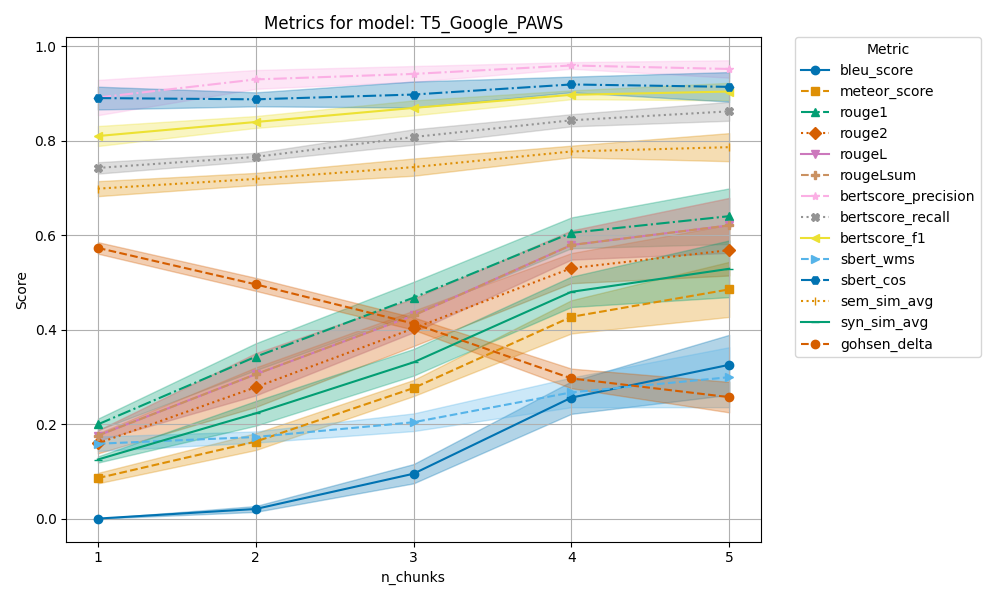
\includegraphics[width=\textwidth]{images/paraphrasing/experiments/T5_Google_PAWS_metrics_plot.png}
    \caption{Average score over different prompts (standard deviation shaded) for different paraphrasing scores for the \ac{t5} model.
    The syntactic scores rise with the number of chunks, while the semantic scores is stable.
    Consequently, the Gohsen Delta score is decreasing with the number of chunks.}
    \label{fig:abl_chunks_T5_Google_PAWS}
\end{figure}

\begin{figure}[htbp]
    \centering
    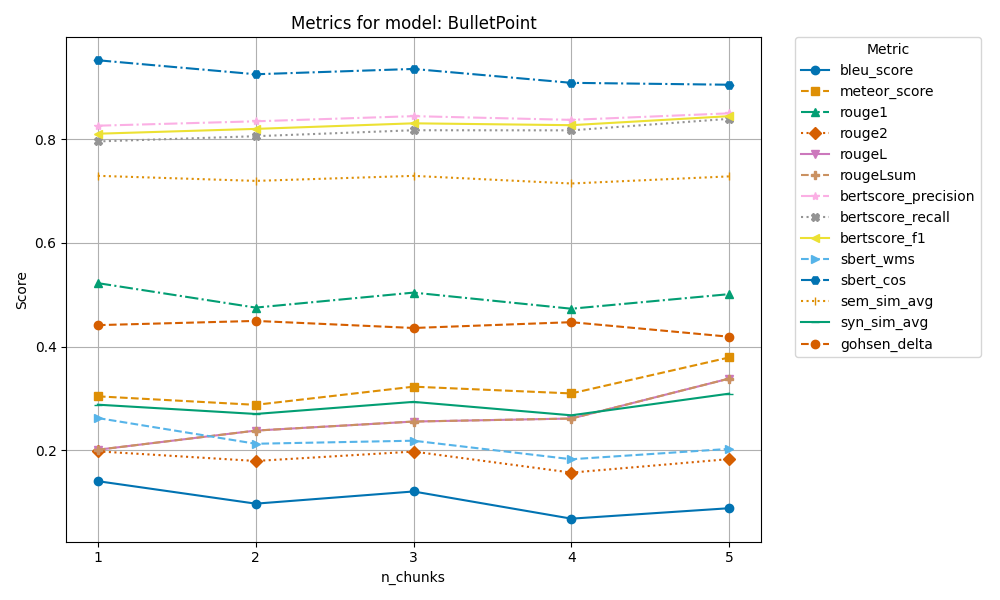
\includegraphics[width=\textwidth]{images/paraphrasing/experiments/BulletPoint_metrics_plot.png}
    \caption{Different paraphrasing scores for the BulletPoint model. 
    This model is not affected by the number of chunks.}
    \label{fig:abl_chunks_BulletPoint}
\end{figure}